\documentclass[10pt,a4paper,titlepage]{article}
\usepackage[a4paper,top=2.5cm,bottom=2.5cm,left=2.5cm,right=2.5cm]{geometry}
%\usepackage{scicite}
\usepackage{times}
\usepackage{hyperref}
\usepackage{setspace}
\usepackage{amsmath}
\usepackage{listings}
\usepackage{graphicx}
\usepackage{enumitem}
\usepackage{tabularx,ragged2e}
\usepackage{geometry}
\usepackage{booktabs}
\usepackage{subcaption}
\usepackage{mwe}

\newcolumntype{L}{>{\RaggedRight\arraybackslash}X}

\makeatletter
\renewcommand*\env@matrix[1][*\c@MaxMatrixCols c]{%
  \hskip -\arraycolsep
  \let\@ifnextchar\new@ifnextchar
  \array{#1}}
\makeatother


\newenvironment{sciabstract}{%
\begin{quote} \bf}
{\end{quote}}



\title{FYS4150 Project 4 - Studies of phase transitions in magnetic systems by numerical implementation of the Ising model} 
\author
{Mikkel Killingmoe Christensen\\
\\
\normalsize{\today}
}


\date{}

%%%%%%%%%%%%%%%%%%%%%%%%%%%%%%%%%%%%%%%%%%%%%%%%%%
%%%%%%%%%%%%%%%%% END OF PREAMBLE %%%%%%%%%%%%%%%%
%%%%%%%%%%%%%%%%%%%%%%%%%%%%%%%%%%%%%%%%%%%%%%%%%%


\begin{document} 


\maketitle 


\tableofcontents
\clearpage


\begin{center}
{\large \textbf{Abstract}}
\end{center}
\begin{sciabstract}
In the early 1900s, a physicist named Ernst Ising created a model explaining the behaviour of phase transitions in magnetic materials in one dimension. The two-dimensional model was later invented by the Norwegian physicist Lars Onsager, and is now known as the Ising model. In this project, the Ising model for a ferromagnetic solid was implemented in a C++ program using the Metropolis algorithm based on Monte Carlo methods. The program was first tested on a 2x2 spin lattice, and compared to known analytical solutions. It was then run on a 20x20 spin lattice to analyse the number of Monte Carlo cycles needed to reach equilibrium of the different properties of the solid. Lastly, the program was run on larger lattices to study the phase transition in the solid, and finally compute the associated critical temperature. The code was found to be fairly accurate compared to analytical results after $10^5$ to $10^6$ Monte Carlo cycles. The critical temperatures calculated from the heat capacity and magnetic susceptibility were found to be $T_{C,C_{V}} \approx$ 2.254 and $T_{C, \chi} \approx$ 2.269. This is close or equal to the temperature Lars Onsager originally found to be $T_C \approx$ 2.269. The temperature calculations were, however, based on a small data set, and more calculations need to be done to conclude. 
\end{sciabstract}




%%%%%%%%%%%%%%%%%%%%%%%%%%%%%%%%%%%%%%
%%%%%%%%%%%Introduction%%%%%%%%%%%%%%%
%%%%%%%%%%%%%%%%%%%%%%%%%%%%%%%%%%%%%%
\section{Introduction}
Magnetic phase transitions have for a long time been an area of interest for researchers because of its strange behaviour, and for its applications in material science. An example of a magnetic phase transition can be seen in so-called ferromagnetic materials. Above a certain temperature called the Curie temperature (denoted $T_C$), the net magnetization is zero due to the random alignment of the spins. If the temperature goes below this, however, the material shows spontaneous magnetization in the absence of an applied magnetic field. This is situation is illustrated in figure (\ref{fig:spin_align}).  

\begin{figure}[ht!]
\centering
\centering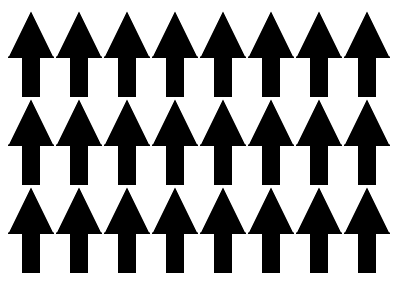
\includegraphics[scale=0.4]{spin_align.png}
\caption{Below a critical temperature $T_C$, magnetic spins in ferromagnetic materials align parallell to each other in the absence of an applied magnetic field. Taken from \cite{spin_align} \label{fig:spin_align}}
\end{figure}

A physicist named Ernst Ising wanted to explain this behaviour with a model, and in 1924 he found a solution for the phase transition in one dimension. The model used was later named the Ising model. The two-dimensional Ising model proved to be much harder to solve, but it was finally done in 1944 by the Norwegian physicist Lars Onsager. This is the version of the model I will implement numerically in this project. The Ising model is chosen because of its simplicity and analytical solutions. Additionally, it is an extremely popular  model with many applications, and it develops intuition about the physics of phase transitions.

The Metropolis algorithm will be used to calculate the properties of the system. It is based on the famous Monte Carlo algorithm, which is a method that needs huge amounts of data to achieve sufficient accuracy. The code should therefore be parallelized using MPI to increase the efficiency of the code, thereby generating more data in less time.  

I will first develop a code that calculates different properties of a simple 2x2 ($L$ = 2) spin lattice using the Ising model, and then compare the results to the analytical values.  Then, the calculations will be repeated for a 20x20 ($L$ = 20) spin lattice. An analysis of the number of Monte Carlo cycles needed to yield sufficient accuracy will be done for both cases. Next, the behaviour of the Ising model close to the critical temperature as a function of lattice size will be investigated. Finally, the critical temperature will be estimated from the data and compared to the exact result.


%%%%%%%%%%%%%%%%%%%%%%%%%%%%%%%%%%%%%%
%%%%%%%%%%%Theory%%%%%%%%%%%%%%%%%%%%%
%%%%%%%%%%%%%%%%%%%%%%%%%%%%%%%%%%%%%%
\section{Theory}
The theory of this project is primarily  based on the lecture notes of Morten Hjort-Jensen \cite{Bok}.

\subsection{The Ising model}
As mentioned, the Ising model will be the basis for this project. 
The model is made up of discrete variables representing magnetic dipole moments of atomic spins. These can be in one of two states (+1 or −1), and they are arranged in a lattice where each spin is allowed to interact with its neighbours. 
	The energy for the system is expressed as
\begin{equation}
E = -J\sum_{<kl>}^{N}s_{k}s_{l}-B\sum_{k}^{N}s_{k},
\end{equation}
where $s = \pm1$ i the direction of the spins, $N$ is the total number of spins, $J$ is the coupling constant giving the strength of the interaction between neighbouring spins and $B$ is an applied external field. The external field will be set to 0 in this project. $<$kl$>$means that the sum only goes over the nearest neighbours of each particle. 

In two dimensions without an external field, the energy is given as
\begin{equation}
\label{eq:L_2_E}
E_i = -J\sum_{k,l=1}^{N}(s_{k,l}s_{k,l+1}+s_{k,l}s_{k+1,l}).
\end{equation}
To make the equation work when the sum approaches $N$, periodic boundary conditions will be introduced. When the end of the lattice is reached, it will jump back to the beginning. 

Summing over all spins of a configuration $i$, we get the magnetization. It is defined as:
\begin{equation}
M_i=\sum_{j=1}^{N}s_{j}.
\end{equation}

\subsection{Calculating properties of the system}
The results from the algorithms in this project will be compared to values from analytical expressions. These will here be derived. 

The Boltzmann distribution is given as: 
\begin{equation}
P_i(\beta)=\frac{e^{-E_i\beta}}{Z},
\end{equation}
where $\beta = \frac{1}{kT}$. $k$ is here the Boltzmann constant, $E_i$ is the energy of state $i$ and $Z$ is the partition function for the canonicle ensemble defined as:
\begin{equation}
\label{eq:partition}
Z = \sum_{i=1}^{M}e^{\beta E_{i}}
\end{equation}
For a canonical ensemble, the expectation value for the energy is defined as
\begin{equation}
\langle E\rangle=k_{b}T^2\left(\frac{\partial lnZ}{\partial T}\right)_{V,N}.
\end{equation}
By instead using the probability distribution, one gets
\begin{equation}
\langle E\rangle=\sum_{i=1}^{M}E_{i}P_{i}(\beta)=\frac{1}{Z}\sum_{i=1}^{M}E_{i}e^{-\beta E_{i}},
\end{equation}
where $M$ is the total number of microstates. 

With a constant volume, the specific heat is given as:
\begin{equation}
\label{eq:spec_heat}
C_{v}=\frac{1}{k_{b}T^{2}}\left(\langle E^2\rangle - \langle E\rangle^2\right).
\end{equation}
The energy terms in equation (\ref{eq:spec_heat}) is also known as the energy variance. It can be calculated as follows:
\begin{equation}
\label{eq:e_var}
\sigma^2_E = \langle E^2\rangle - \langle E\rangle^2 = \frac{1}{Z}\sum_{i=1}^{M}E_i^2e^{-\beta E_i}-\left(\frac{1}{Z}\sum_{i=1}^{M}E_ie^{-\beta E_i}\right)^{2}
\end{equation}
The magnetization has the following expression for the expectation value:
\begin{equation}
\langle M\rangle = \sum_i^{M}M_{i}P_{i}=\frac{1}{Z}\sum_i^{M}M_{i}e^{-\beta E_i}.
\end{equation}
This formula will, however, not be used since it yields a magnetization of zero for a square lattice. Instead, the expectation value of the absolute value of the magnetization will be used. It is given as:
\begin{equation}
\label{eq:magn}
\langle |M|\rangle = \sum_i^{M}|M|_{i}P_{i}=\frac{1}{Z}\sum_i^{M}|M|_{i}e^{-\beta E_i}.
\end{equation}
Lastly, the magnetic susceptibility of the system is given as:
\begin{equation}
\chi = \frac{1}{k_{b}T}\left(\langle M^2\rangle-\langle|M|\rangle^2\right).
\end{equation}

\subsection{Analytical solution of the Ising model for L = 2}
An analytical solution for a $L$ = 2 Ising model case will now be derived. These values will be divided by the total number of spins when used in the final comparison with the numerical results. Periodic boundary conditions will also be used. 

The energy for this system is given by equation (\ref{eq:L_2_E}). 
The combinations of spins and their respective energies are then:
\begin{equation}
E = -8J, \bigg\{
  \begin{pmatrix}
    \uparrow & \uparrow \\
    \uparrow & \uparrow
  \end{pmatrix},
  \begin{pmatrix}
    \downarrow & \downarrow \\
    \downarrow & \downarrow
  \end{pmatrix} \bigg\}
\end{equation}

\begin{equation}
E = +8J, \bigg\{
  \begin{pmatrix}
    \downarrow & \uparrow \\
    \uparrow & \downarrow
  \end{pmatrix},
  \begin{pmatrix}
    \uparrow & \downarrow \\
    \downarrow & \uparrow
  \end{pmatrix} \bigg\}
\end{equation}

\begin{equation}
E = 0, \bigg\{
\begin{pmatrix}
    \uparrow & \downarrow \\
    \downarrow & \downarrow
  \end{pmatrix},
  \begin{pmatrix}
    \downarrow & \uparrow \\
    \uparrow & \uparrow
  \end{pmatrix},
  \begin{pmatrix}
    \downarrow & \downarrow \\
    \uparrow & \uparrow
  \end{pmatrix}
   \bigg\}
\end{equation}
All the possible configurations are also presented in table (\ref{tab:conf}).
\begin{table}[!ht]
\centering
\caption{All the possible configurations for a $L$ = 2 lattice. The energy and magnetizations vary as a function of the number of spins pointing up. } \label{tab:conf}
\begin{tabular}{| c | c | c | c |} \hline
\textbf{Spins up} & \textbf{Degeneracy} & \textbf{Energy} & \textbf{Magnetization} \\ \hline
4 & 1 & -8J & 4 \\ \hline
3 & 4 & 0 & 2 \\ \hline
2 & 4 & 0 & 0 \\ \hline
2 & 2 & +8J & 0 \\ \hline
1 & 4 & 0 & -2 \\ \hline
0 & 1 & -8J & -4 \\ \hline
\end{tabular}
\end{table}
It is now easy to calculate the different analytical values using the equations presented earlier. 

First, the partition function is calculated using equation (\ref{eq:partition}). By summing all the possible energies, I get that\footnote{where I have used that $cosh(x) = ( e^x + e^{-x} )/2$}:
\begin{equation}
Z = \sum_{i=1}^{M}e^{-\beta JE_{i}} = 2e^{-8J\beta}+2e^{8J\beta}+12e^{0\beta} = 4 cosh(8J\beta)+12
\end{equation}
The energy then becomes\footnote{where I have used that $sinh(x) = ( e^x - e^{-x} )/2$}:
\begin{equation}
\langle E\rangle=\frac{16J(e^{-8J\beta}-e^{8J\beta})}{Z}=\frac{-32J}{Z}sinh(8J\beta)
\end{equation}
The heat capacity can now be calculated using the equations for the energy variance and specific heat:
\begin{equation}
C_v = \frac{1}{k_{b}T^2}\left(\frac{(16J)^{2}cosh(8J\beta)}{Z}-\left(-\frac{32Jsinh(8J\beta)}{Z}\right)^{2}\right)
\end{equation}
The mean magnetization can be calculated by using equation (\ref{eq:magn}):
\begin{equation}
\langle|M|\rangle = \frac{1}{Z}\left(4e^{8J\beta}+4e^{8J\beta}+8e^{-0J\beta}+8e^{-0J\beta}\right)=\frac{1}{Z}\left(8e^{8J\beta}+16\right).
\end{equation}
Lastly, the susceptibility can be calculated from the magnetization:
\begin{equation}
\chi = \frac{1}{k_{b}T}\left(\langle M^2\rangle-\langle|M|\rangle^2\right)=\frac{1}{k_{b}T}\left(\frac{32}{Z}\left(e^{8J\beta}+1\right)-\frac{1}{Z^{2}}\left(8e^{8J\beta}+16\right)^{2}\right)
\end{equation}


%%%%%%%%%%%%%%%%%%%%%%%%%%%%%%%%%%%%%%
%%%%%%%%%%%Method%%%%%%%%%%%%%%%%%%%%%
%%%%%%%%%%%%%%%%%%%%%%%%%%%%%%%%%%%%%%
\section{Method}
\subsection{The Metropolis algorithm}
The Metropolis algorithm based on the Monte Carlo method will in this project be used to implement the Ising model numerically in C++. The algorithm was originally invented by Nicholas Metropolis 1953, and later generalized by W.B. Hastings in 1970 \cite{metro}.

The algorithms works by using Monte Carlo methods on Markov chains. In a nutshell, a random state is chosen and changed from $x$ to $x'$, but is only accepted if it moves towards and equilibrium. The algorithms consists of the steps shown below. This is defined as one Monte Carlo cycle. After the algorithm is run, the expectation values should be divided by the total number of cycles. 

The coupling constant $J$ and the Boltzmann constant $k_B$ were both set to 1. 

\paragraph{The Metropolis algorithm}
\begin{enumerate}
  \item Initial state of spin configurations is set up in a matrix, \textbf{s}. A corresponding initial energy $E_0$ is defined.
  \item A spin state, $s_{ij}$, is picked randomly and flipped.
  \item The change in energy from the flip, $\Delta E$, is calculated.
  \item If $\Delta E < 0$, the new configuration is accepted and we can proceed to point 6. 
  \item If $\Delta > 0$, calculate $w = e^{-\beta\Delta E}$. Then compare $w$ to a random number $r \in[0,1]$. If $r\leq w$, the configuration is accepted. 
  \item Update all the expectation values.
  \item Repeat steps 2-6 until equilibrium is reached. 
\end{enumerate}

\subsection{The critical temperature}
One goal of the project is to estimate the critical temperature (Curie temperature) of the system. It is possible to find it through the use of finite size scale relations \cite{project}. This can relate behaviour of finite size lattices with results from an infinitely large lattice. The critical temperature scales as:
\begin{equation}
T_{C}(L)-T_{C}(L=\infty)=\alpha L^{-\frac{1}{\nu}}=\frac{\alpha}{L},
\end{equation}
where $T_C(L)$ is the critical temperature for a given lattice with size $L$x$L$, $T_{C}(L=\infty)$ is the critical temperature when for a lattice with a size approaching  infinity, $\alpha$ is a proportionality constant and $\nu$ is set to 1. Solving for $T_C(L=\infty$) can be done numerically by running the algorithm for different values of $L$, returning values for $T_C(L)$. $T_C(L=\infty)$ is then given by:
\begin{equation}
\label{eq:crit}
T_C(L=\infty) = \frac{1}{N}\sum_{i\neq j}\frac{L_iT_C(L_i)-L_jT_C(L_j)}{L_i-L_j}.
\end{equation}
Here, the sum goes over all the different combinations of $L_i$ and $L_j$. It is then divided by the total number of combinations, $N$.

Lars Onsager found this to be approximately $T_C \approx$ 2.269 \cite{onsanger}. 


%%%%%%%%%%%%%%%%%%%%%%%%%%%%%%%%%%%%%%
%%%%%%%%%%%Results%%%%%%%%%%%%%%%%%%%%
%%%%%%%%%%%%%%%%%%%%%%%%%%%%%%%%%%%%%%
\section{Experimental}
The code used in this project can be found at the GitHub repository below:

\par \url{https://github.com/mikkello/FYS4150/}

\subsection{Comparison of numerical results to analytical values}
A code for the Ising model (main.cpp) was written and first tested with a $L = 2$ lattice to see if the program run as expected, and gave results comparable to the analytical benchmarks. The algorithm was run with a temperature $T$ = [1, 3] with $\Delta T$ = 0.1, and it calculated the previously  mentioned properties. An analysis of the number of Monte Carlo cycles needed to achieve good agreement was done. 

\subsection{Thermalization}
To have a more realistic representation of a solid, the code was run for a lattice with $L=20$ in both directions. The mean energy, mean magnetization, heat capacity and magnetic susceptibility as functions of the number of Monte Carlo cycles were plotted. The number of cycles were used as a representation of time. A temperature of $T = 1.0$ was first used to study the mean energy and magnetization with both ordered and random initial spin configurations. It was then repeated for $T = 2.4$. 

An analysis of the number of Monte Carlo cycles needed to reach equilibrium were done, and based on this, the equilibration time were estimated. Additionally, a plot of the normalized number of accepted configurations as a function of the total number of Monte Carlo cycles were made. 

\subsection{Analysing the probability distribution}
To analyse the probability distribution, the probability $P(E)$ for the $L=20$ system were computed at the same temperatures after a steady state situation was reached. This was done by counting the number of times a specific energy $E$ appeared in the data set.  The variance was computed from the probability distribution, and was then compared to the computed variance from the heat capacity data using equation (\ref{eq:spec_heat}). 

\subsection{Study of phase transitions}
After the probability analysis, the behaviour of the Ising model in two dimensions as a function of lattice size was studied close to the critical temperature. The various properties of the system was calculated as functions of temperature for $L=[40,60,80,100]$ with $T\in[2.15,2.35]$ and $10^5$ Monte Carlo cycles in steps of $\Delta T = 0.05$. The results were then plotted. Using this data, two values for the critical temperature were extracted by using data from the peaks of the heat capacity and the magnetic susceptibility respectively. 

Parallelization with MPI was meant to be used in this part to generate more data and thereby finding a more accurate critical temperature. There was, however, no speed-up after implementing the parallelization, indicating a problem with the implementation of the MPI library or with settings in Visual Studio or Windows. Smaller time steps and more Monte Carlo cycles would be used without this problem. 


%%%%%%%%%%%%%%%%%%%%%%%%%%%%%%%%%%%%%%
%%%%%%%%%%%Results%%%%%%%%%%%%%%%%%%%%
%%%%%%%%%%%%%%%%%%%%%%%%%%%%%%%%%%%%%%
\section{Results}
\subsection{Comparison of numerical results to analytical values}
The first goal of the project was to test the code on a $L$ = 2 spin lattice to see how many Monte Carlo cycles were needed to achieve sufficient accuracy.
	In table (\ref{tab:num_vs_ana}), a comparison of the analytical values to the numerical values for $10^4$, $10^5$ and $10^6$ Monte Carlo cycles at a temperature of $T$ = 1 can be seen. 
	In figure (\ref{fig:b_rel_err}), a plot of the relative error as a function of the number of Monte Carlo cycles is shown. 
	On the basis of the results in figure (\ref{fig:b_rel_err}), $10^6$ cycles were chosen when plotting the numerical and analytical mean energy, mean magnetization, heat capacity and susceptibility as a function of temperature in figure (\ref{fig:b_Num_vs_Ana}). 
	
\begin{table}[ht!]
\centering
\caption{Comparing the analytical values to the numerical values for $10^4$, $10^5$ and $10^6$ Monte Carlo cycles (MCCs) at a temperature of 1 ($L$ = 2). As expected, the values become more accurate by increasing the number of Monte Carlo cycles.  } \label{tab:num_vs_ana}
\begin{tabular}{| c | c | c | c | c |} \hline
 & \textbf{Analytical} & \textbf{Numerical ($10^4$ MCCs)} & \textbf{Numerical ($10^5$ MCCs)} & \textbf{Numerical ($10^6$ MCCs)} \\ \hline
$\langle E \rangle$ & -1.995982 & -1.9957 & -1.99572 & -1.99597\\ \hline
$\langle |M| \rangle$ & 0.998661 & 0.998525 & 0.998542 & 0.998664\\ \hline
$C_v$ & 0.032082 & 0.034326 &0.0341667 & 0.032215\\ \hline
$\chi$ & 0.0040107 & 0.0043413 & 0.0044165& 0.00396086\\ \hline

\end{tabular}
\end{table}

\begin{figure}[]
\centering
\centering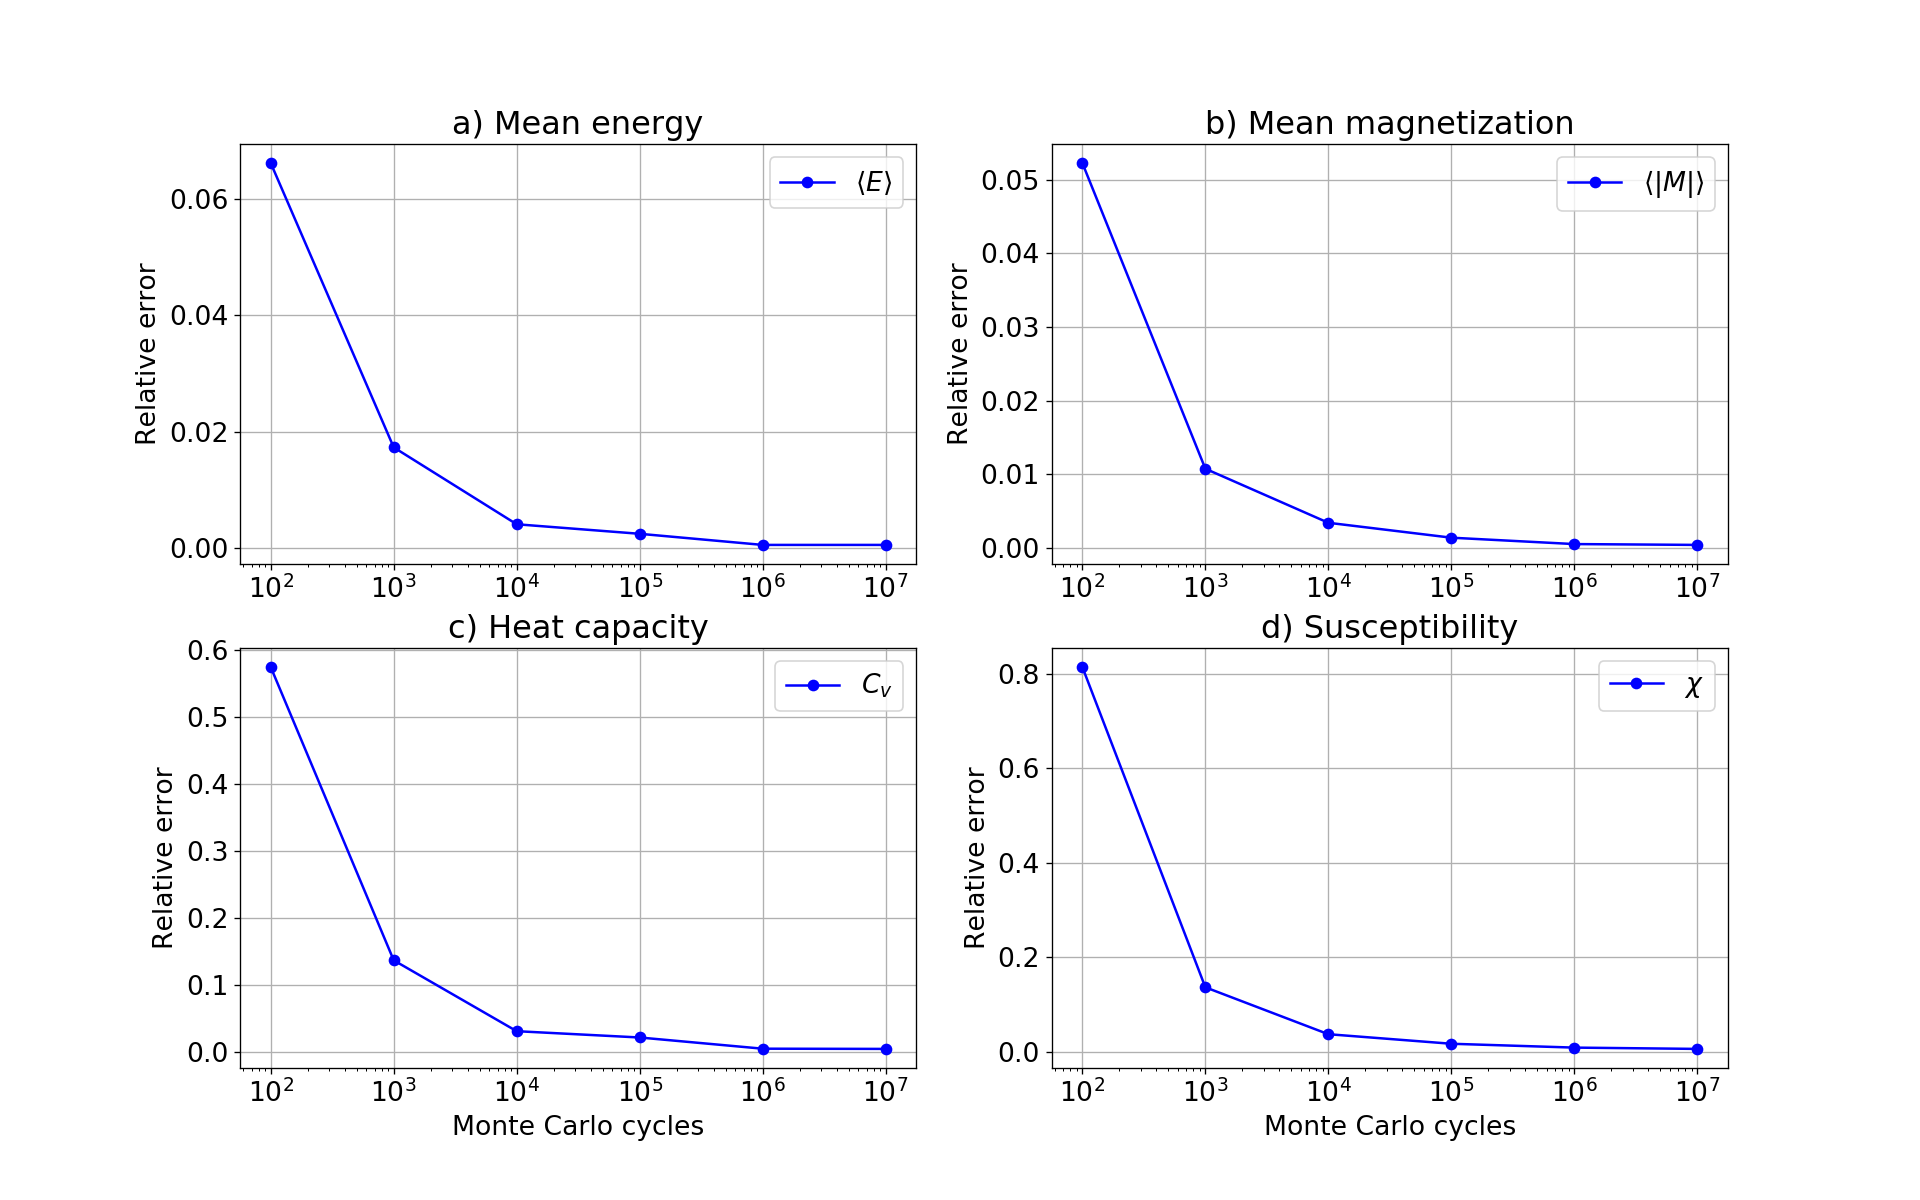
\includegraphics[scale=0.3]{relerr_T10.png}
\caption{Plots of the relative error of the mean energy (a), mean magnetization (b), heat capacity (c) and magnetic susceptibility (d) as a the number of Monte Carlo cycles for a $L$ = 2 spin lattice. The graphs show that $10^5$ to $10^6$ Monte Carlo cycles are needed to achieve good agreement with analytical values.  \label{fig:b_rel_err}}
\end{figure}

\begin{figure}[]
\centering
\centering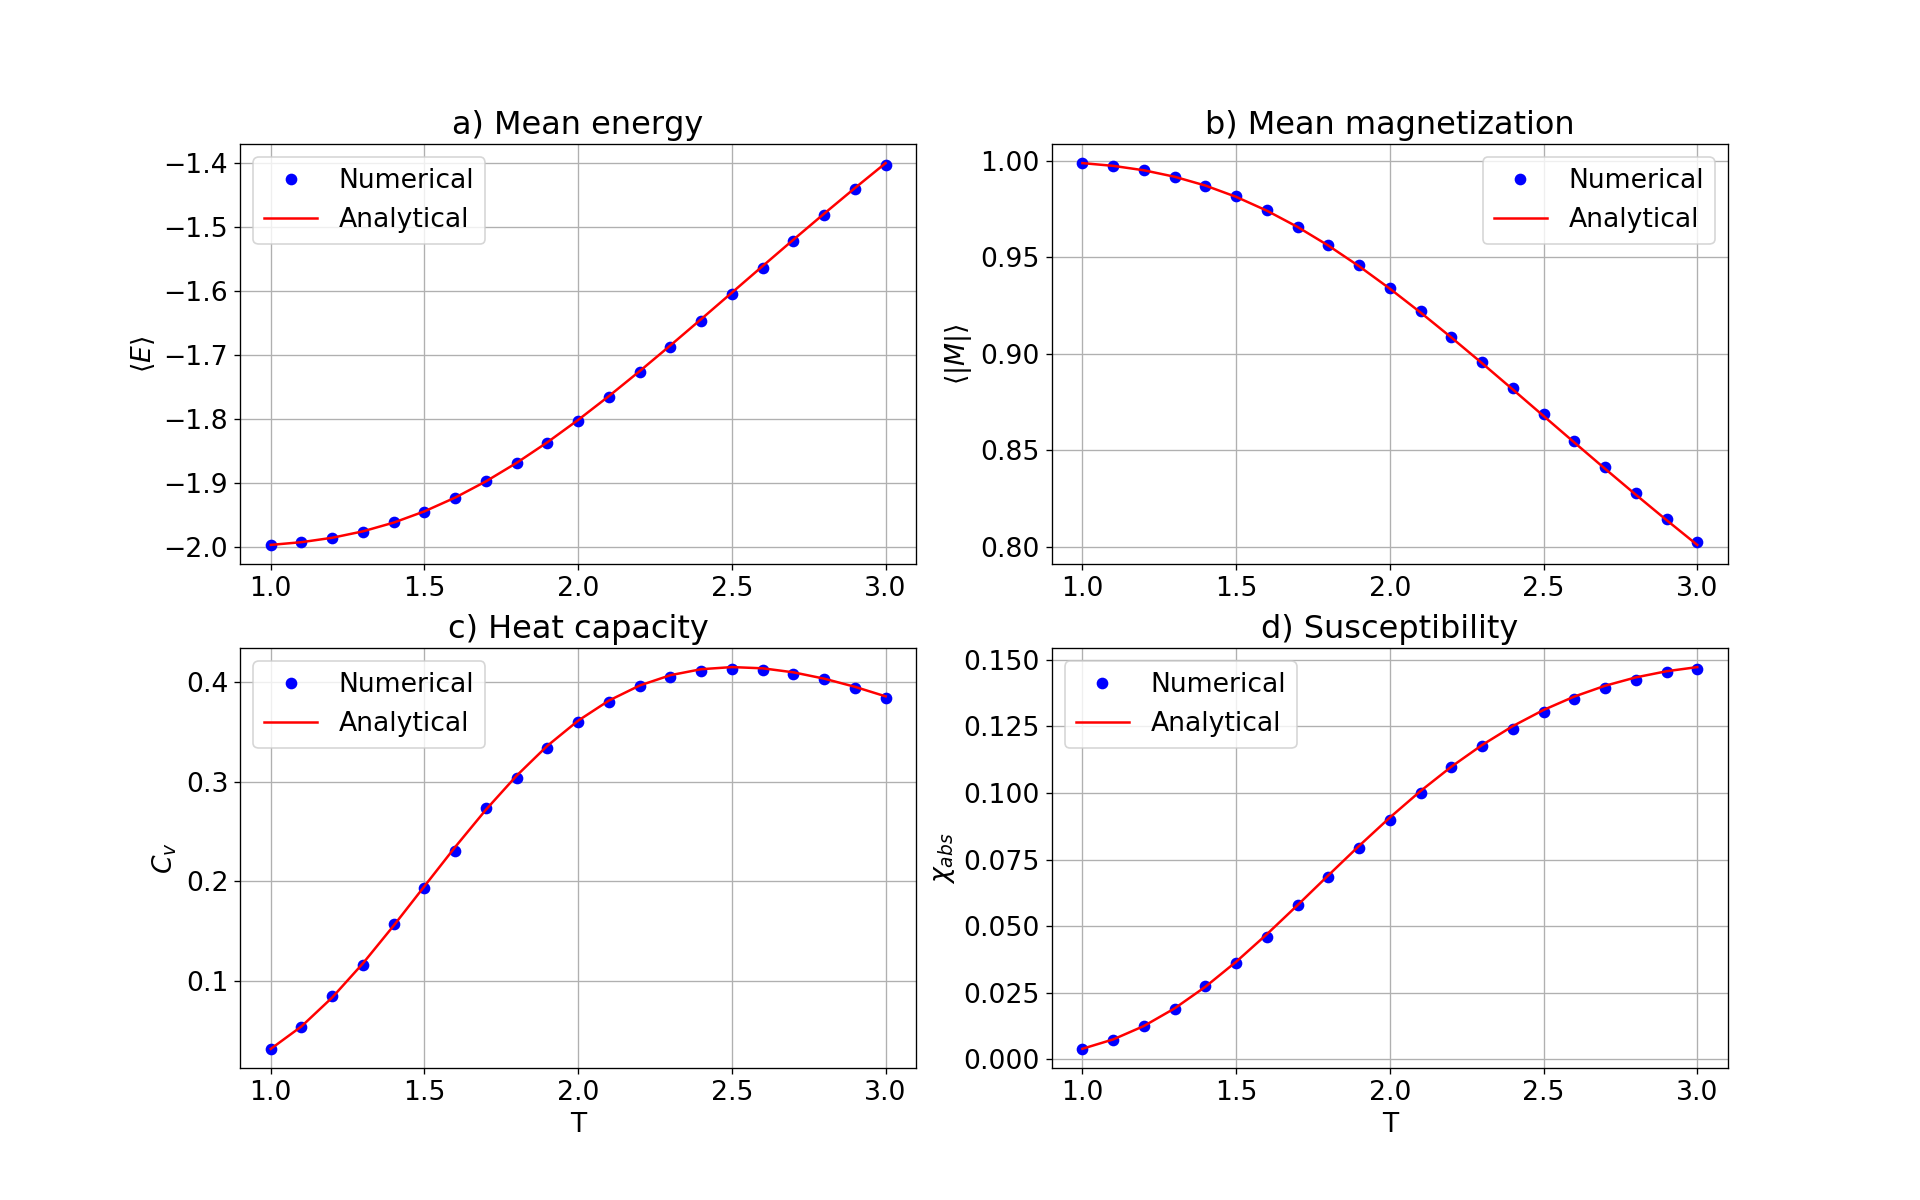
\includegraphics[scale=0.3]{L2_1E+06.png}
\caption{Plots of mean energy (a), mean magnetization (b), heat capacity (c) and magnetic susceptibility (d) as a function of temperature. The blue dots represent the numerical values, while the red lines represent the analytical values. The data was computed using $10^6$ Monte Carlo cycles on a spin matrix with size $L$ = 2. The numerical values are in good agreement with the analytical values for $10^6$ Monte Carlo cycles. \label{fig:b_Num_vs_Ana}}
\end{figure}






\subsection{Thermalization}
The next goal was to find the number of Monte Carlo cycles needed to achieve equilibrium of the different properties of $L$ = 20 lattices with ordered and random initial spin configurations. In figure (\ref{fig:c_thermal}), a plot showing these properties as a function of number of Monte Carlo cycles for $T$ = 1 and $T$ = 2.4 can be seen. 


	

\begin{figure}[]
\centering
\centering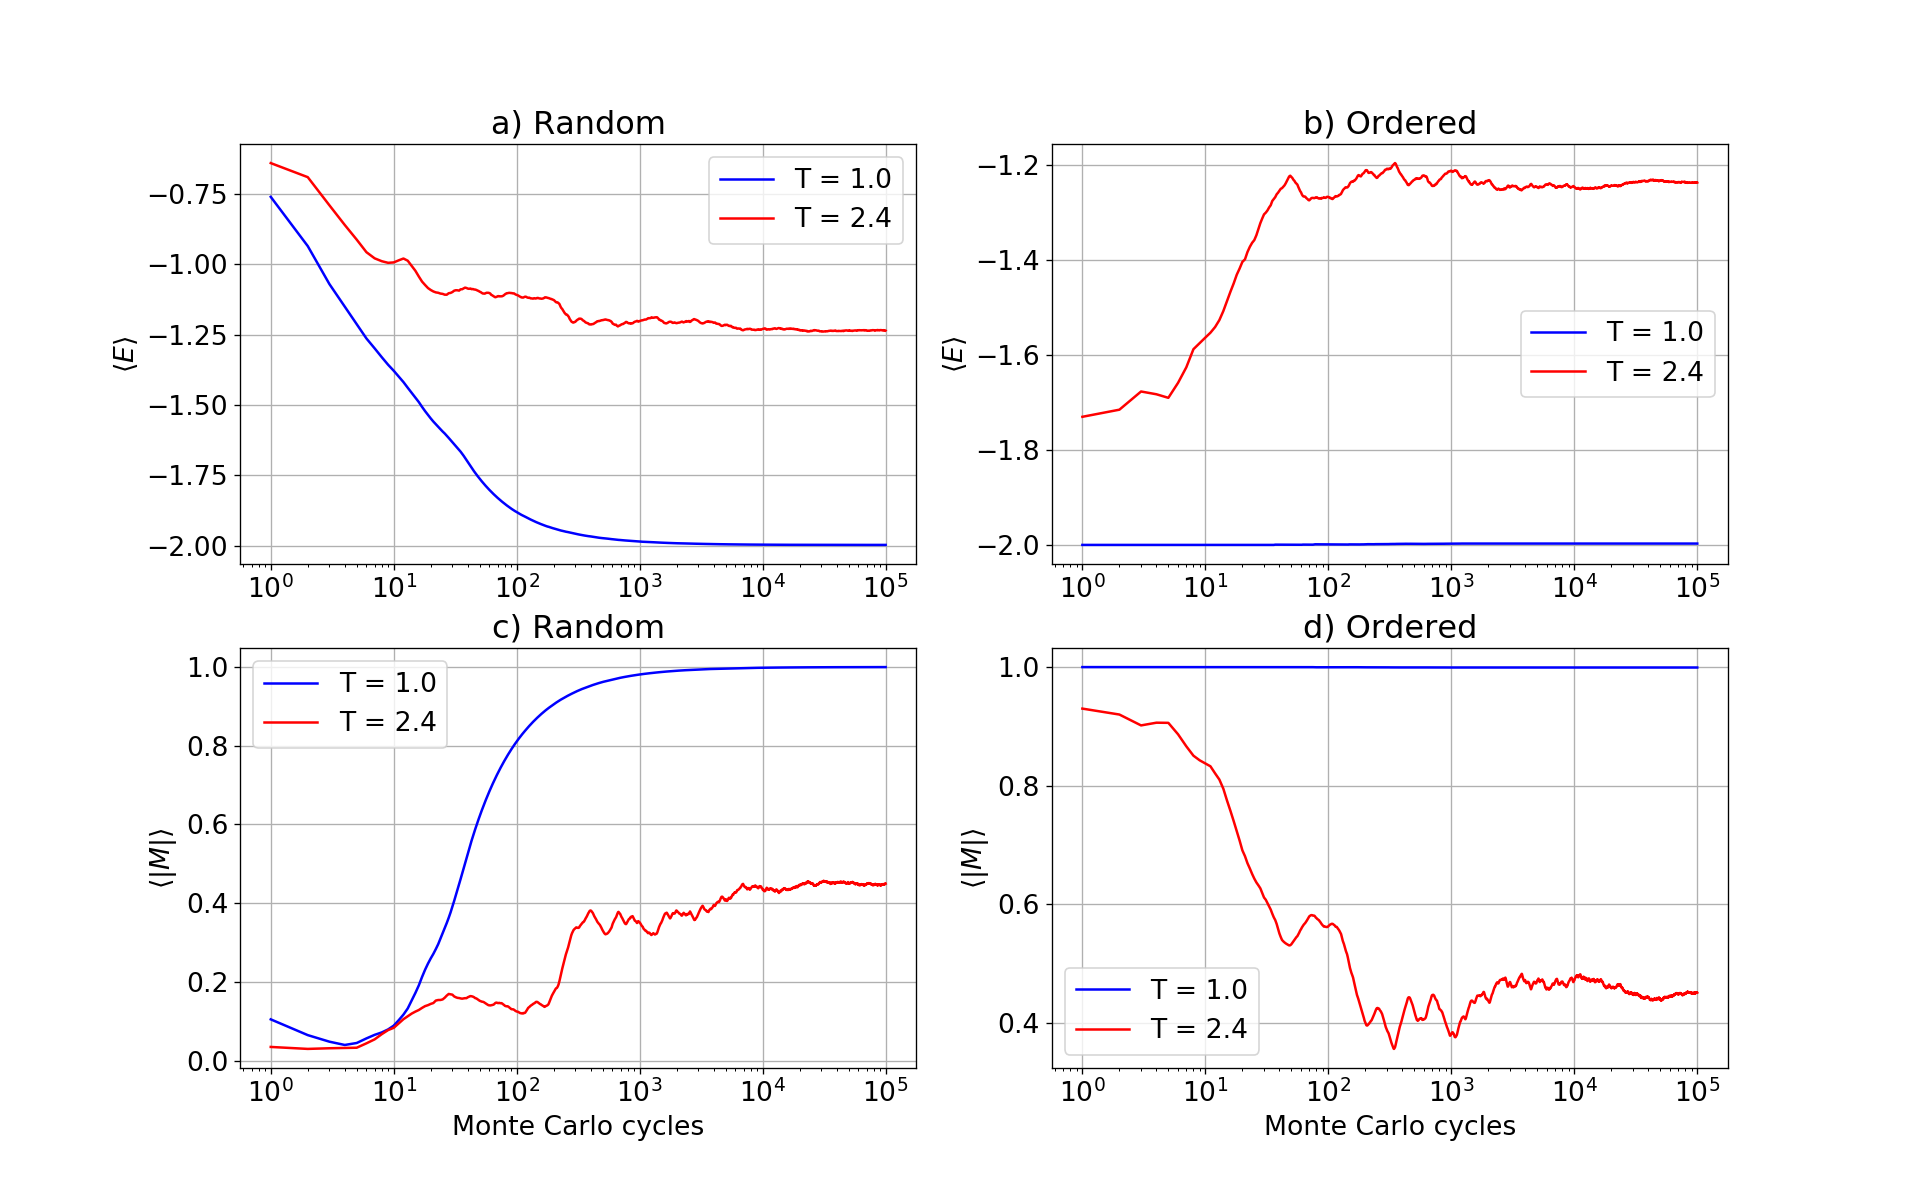
\includegraphics[scale=0.3]{taskc_1.png}
\caption{Plots of the mean energy (a and b) and the mean magnetization (c and d) as a function of the number of Monte Carlo cycles. The calculations were done for $T$ = 1 and $T$ = 2.4 with both random (left) and ordered (right) $L$ = 20 intital spin matrices. For all situations, the values start to stabalize around $10^3$ Monte Carlo cycles, exept for $T$ = 1 whit an ordered intital spin matrix. Another difference is the greater amount of fluctuations at higher temperatures.    \label{fig:c_thermal}}
\end{figure}

Analyses of the normalized number of accepted configurations were also done. In figure (\ref{fig:c_accepted_MCC}), a plot of the normalized number of accepted configurations can be seen as a function of the number of Monte Carlo cycles for $T$ = 1.0 and $T$ = 2.4. In figure (\ref{fig:c_accepted_T}), a plot of the normalized number of accepted configurations as a function of temperature is shown.

\begin{figure}[]
\centering
\centering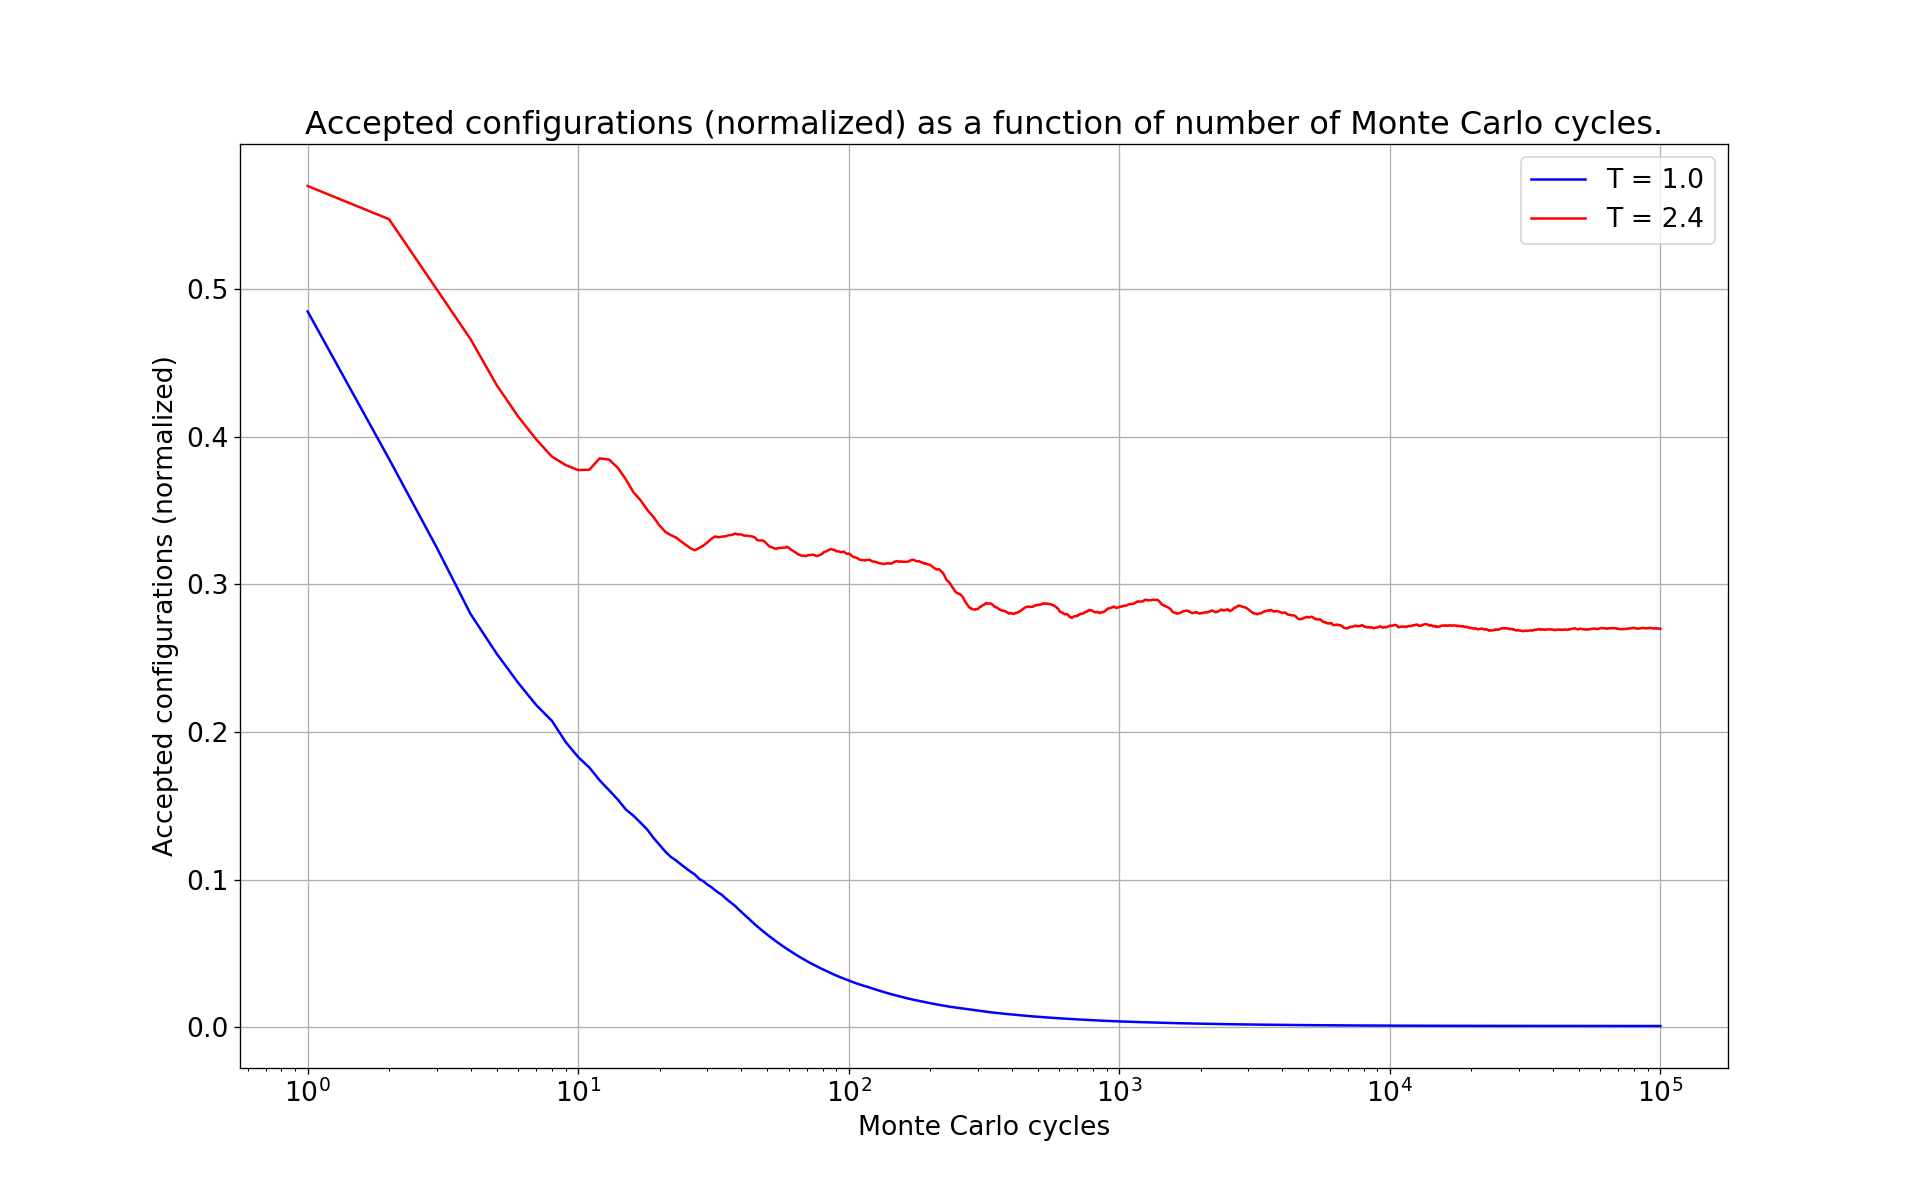
\includegraphics[scale=0.3]{taskc_2.png}
\caption{Plot of the normalized number of accepted configurations as a function of the number of Monte Carlo cycles for $T$ = 1.0 and $T$ = 2.4 on a $L$ = 20 spin matrix. As in figure (\ref{fig:c_thermal}), there are more fluctuations at the higher temperature. The calculation done on the higher temperature does also have more accepted configurations. Both graphs stabalize at around $10^3$ Monte Carlo cycles.  \label{fig:c_accepted_MCC}}
\end{figure}

\begin{figure}[]
\centering
\centering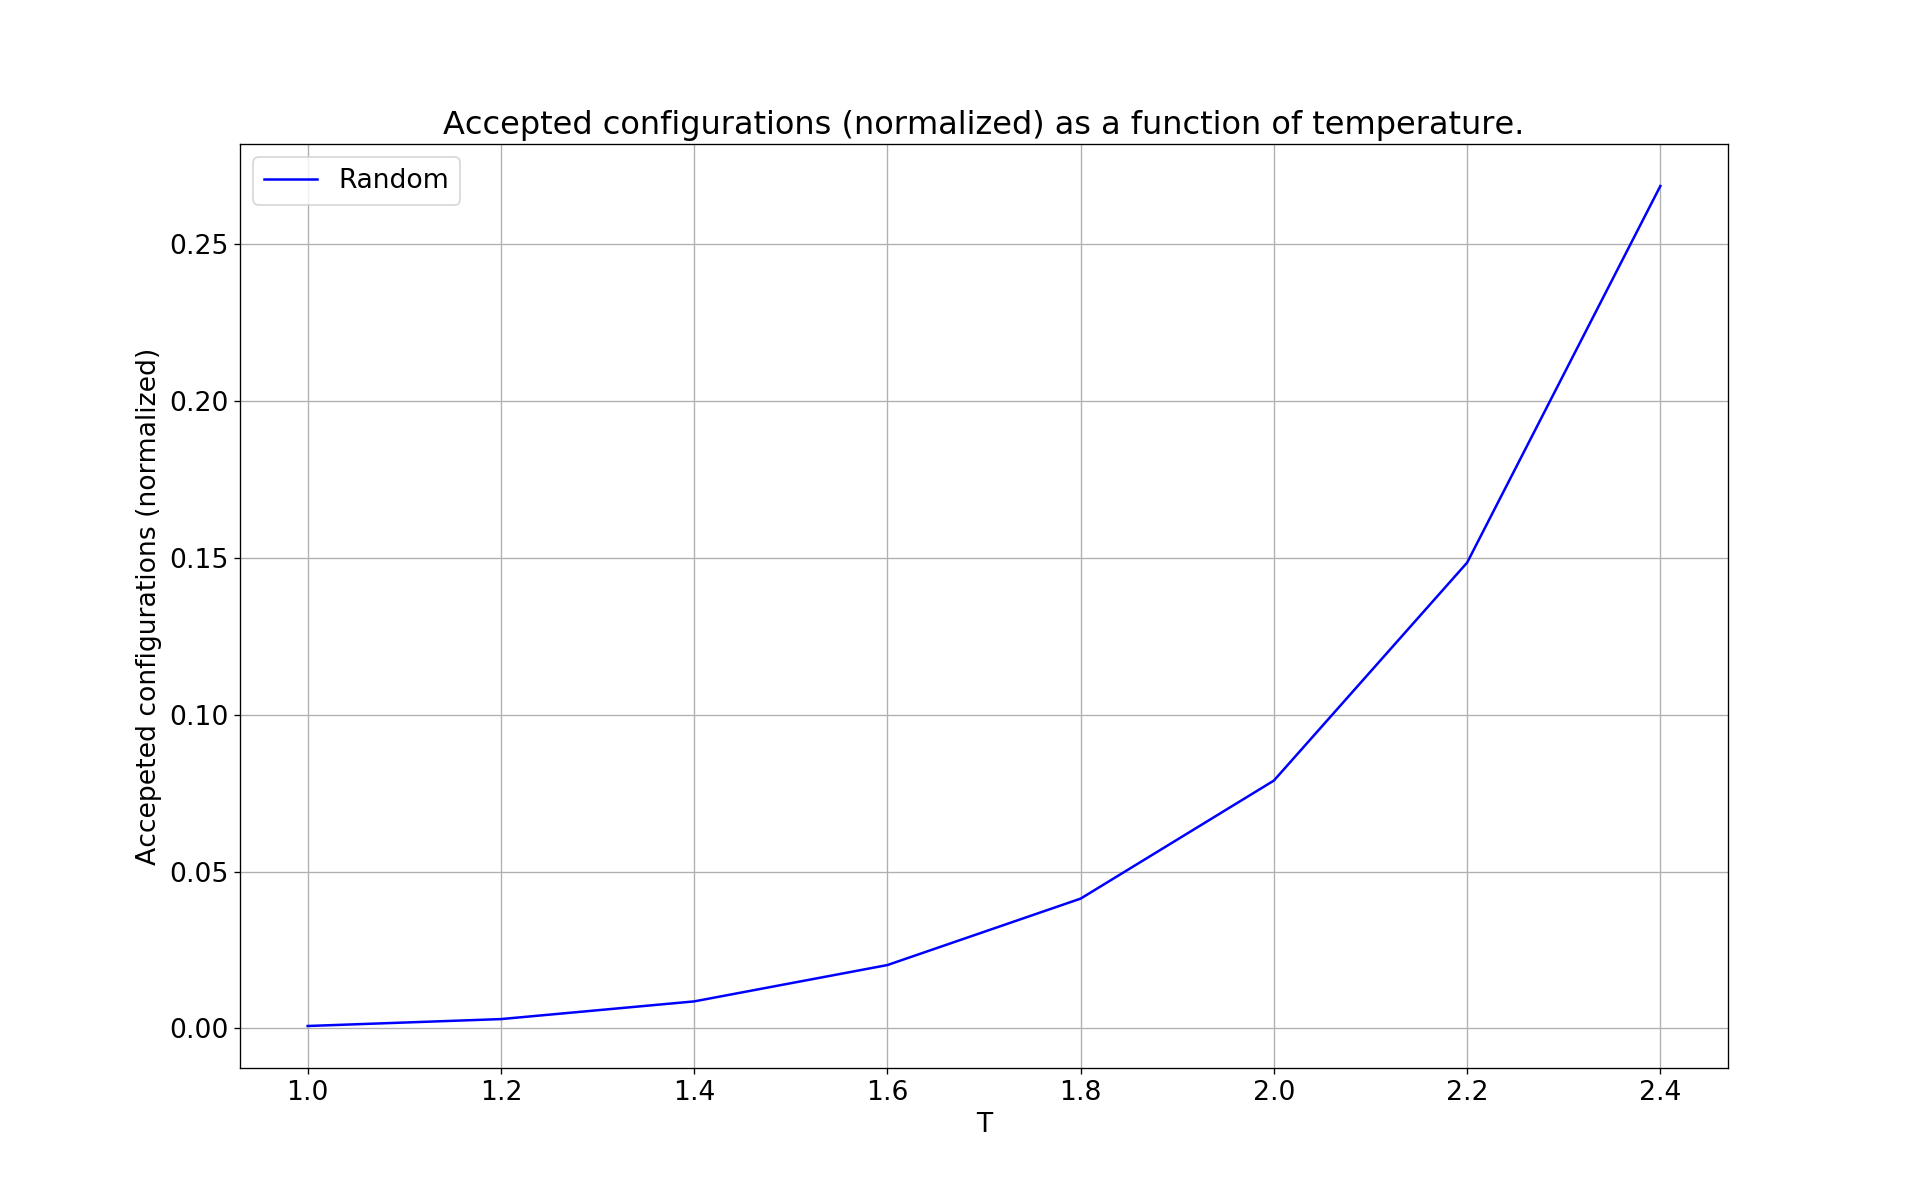
\includegraphics[scale=0.3]{taskc3_acc_vs_T_L20_1e5.png}
\caption{Plot of the normalized number of the accepted configurations as a function of temperature for a $L$ = 20 spin matrix. This plot confirms the trend seen in figure (\ref{fig:c_accepted_MCC}). The number of accepted configurations increases with increasing temperature.   \label{fig:c_accepted_T}}
\end{figure}

\subsection{Probability distribution}
The probability distribution for the energy of $L$ = 20 spin matrices at $T$ = 1 and $T$ = 2.4 with random initial spin states can be seen in figure (\ref{fig:d_prob}). The calculated expectation value is represented by a red line, and the standard deviation calculated using equation (\ref{eq:spec_heat}) is represented by the green lines. 
The variances from the mentioned equation and from the dataset is presented in table (\ref{tab:d_variance}).

\begin{figure}[]
\centering
\centering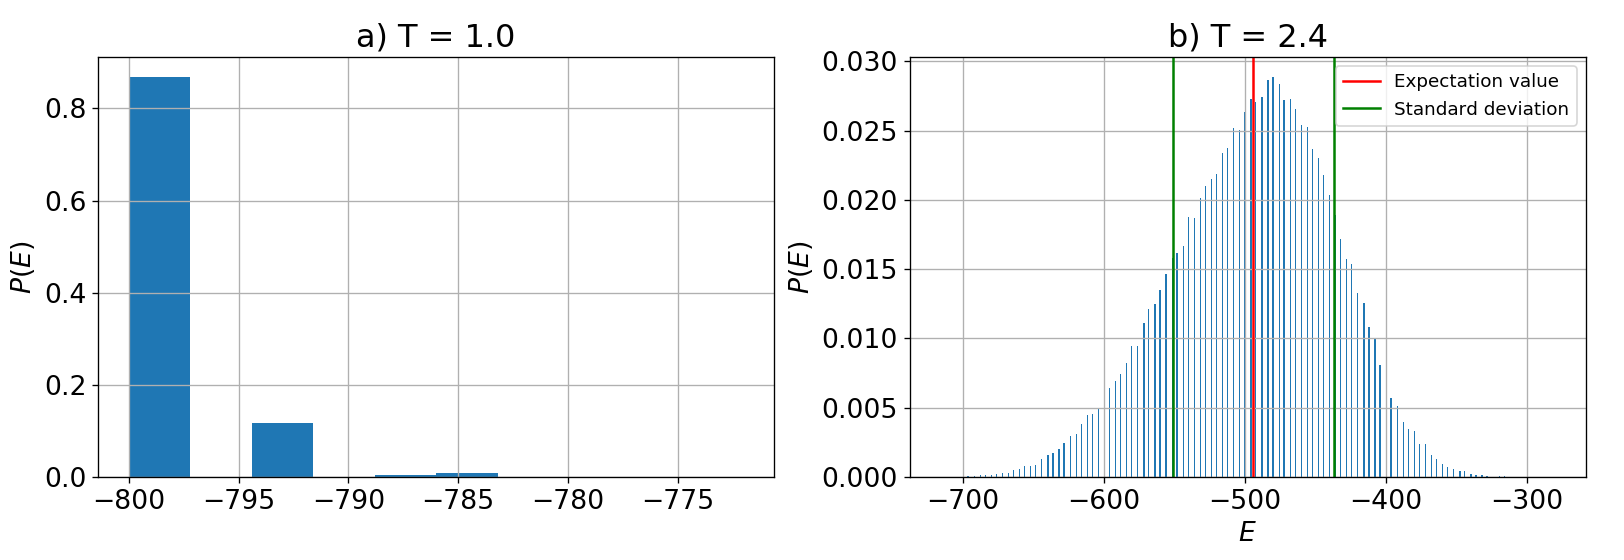
\includegraphics[scale=0.4]{taskd_P(E)_vs_E_1e5_L20.png}
\caption{Histograms for the probability of energy dispersion in $L$ = 20 matrices for $T$ = 1.0 (a) and $T$ = 2.4 (b). The calculated expectation value and standard deviation (from equation (\ref{eq:spec_heat}) is shown in red and green respectively. As seen in the plots, the distribution of energies is much wider for the higher temperature. $10^5$ Monte Carlo cycles were used in the calculations.   \label{fig:d_prob}}
\end{figure}

\begin{table}[ht!]
\centering
\caption{Comparing variances for $T$ = 1 and $T$ = 2.4. The values are calculated from the heat capacity equation (\ref{eq:spec_heat}) and from the dataset shown in figure (\ref{fig:d_prob}) using a variance function in Python. The values are reasonably close to each other.} \label{tab:d_variance}
\begin{tabular}{| c | c | c |} \hline
 & $\mathbf{\sigma_E^2/L^2, T}$ \textbf{= 1.0} & $\mathbf{\sigma_E^2/L^2, T}$ \textbf{= 2.4} \\ \hline
From variance equation & 0.0232 & 8.136\\ \hline
From data set & 0.0239 & 8.087\\ \hline


\end{tabular}
\end{table}

\subsection{Phase transitions}
The final goal of the project was to find a value for the critical temperature of the system and compare this to the Onsager value $T_C \approx2.269$.
	In figure (\ref{fig:phase}) plots of the mean energies, mean magnetizations, heat capacities and susceptibilities for spin matrices with sizes $L$ = [40, 60, 80, 100] as a function of temperature can be seen. The top points of the heat capacity and susceptibility graphs were found, and they are presented in table (\ref{tab:critical_temp}).
These values can give an estimate to the critical temperature of the phase transition using equation (\ref{eq:crit}). Using this equation on the values yielded the critical temperatures of $T_{C,C_{V}} \approx$ 2.254 and $T_{C, \chi} \approx$ 2.269. 




\begin{figure}[]
\centering
\centering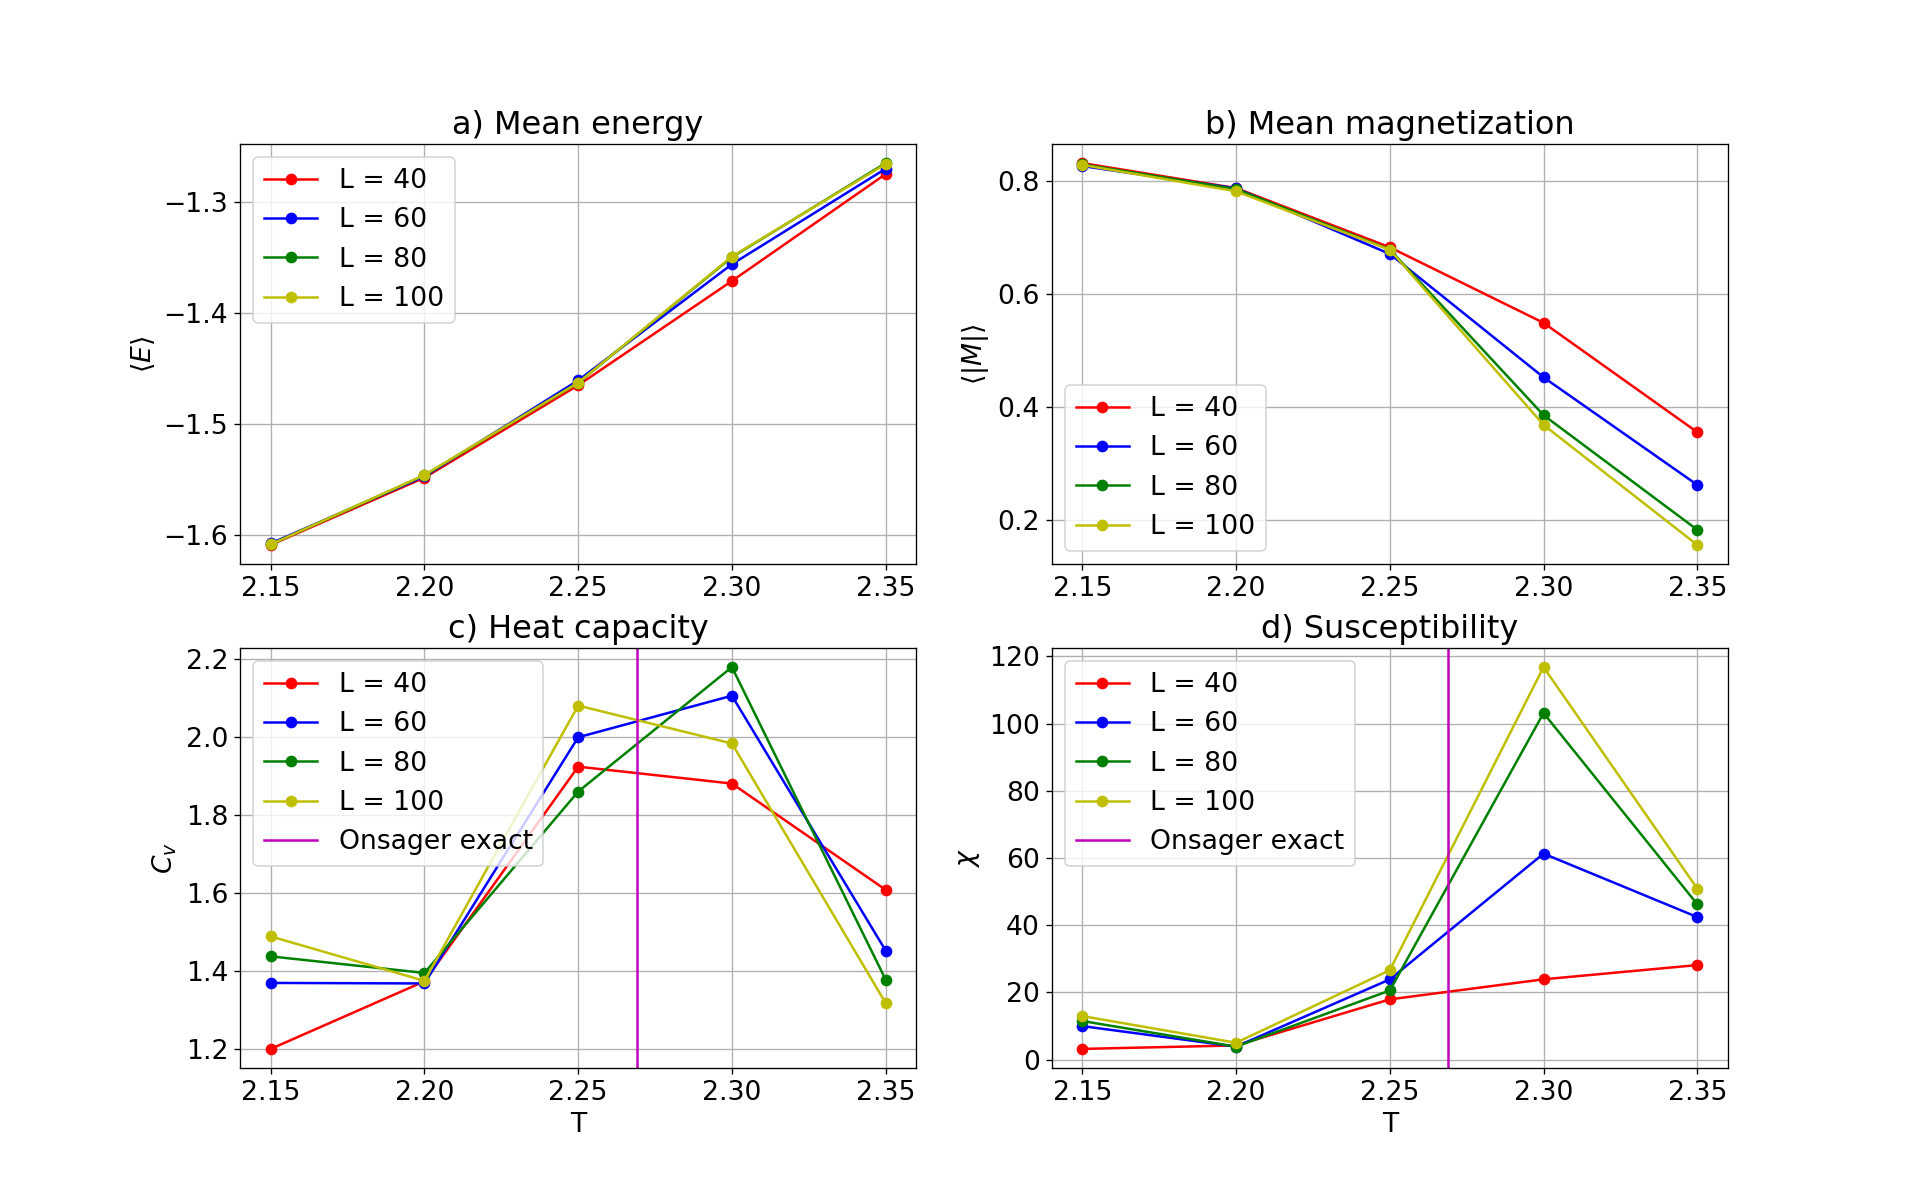
\includegraphics[scale=0.3]{e_L_40_100.png}
\caption{Plots of the mean energy (a), mean magnetization (b), heat capacity (c) and susceptibility (d) for spin matrices with sizes $L$ = [40, 60, 80, 100] as a function of temperature. The calculations were done close to the critical temperature with $10^5$ Monte Carlo cycles and $\Delta T$ = 0.05. The Onsager exact temperature is plotted in pink. In both the heat capacity plot and susceptibility plot, a peak becomes increasingly more visible with increasing lattice size. This is a good indication of the phase transition. \label{fig:phase}}
\end{figure}

\begin{table}[ht!]
\centering
\caption{The calculated temperatures from the top points of the heat capacities and susceptibilites from (figure (\ref{fig:phase}) c and d). } \label{tab:critical_temp}
\begin{tabular}{| c | c | c |} \hline
\textbf{L} & $\mathbf{T_{C, max}}$ from $\mathbf{C_v}$ & $\mathbf{T_{\chi, max}}$ from $\mathbf{\chi}$  \\ \hline
40 & 2.25 & 2.35 \\ \hline
60 & 2.30 & 2.30 \\ \hline
80 & 2.30 & 2.30 \\ \hline
100 & 2.25 & 2.30 \\ \hline
\end{tabular}
\end{table}
%%%%%%%%%%%%%%%%%%%%%%%%%%%%%%%%%%%%%%
%%%%%%%%%%%Discussion%%%%%%%%%%%%%%%%%
%%%%%%%%%%%%%%%%%%%%%%%%%%%%%%%%%%%%%%
\section{Discussion}
\subsection{Comparison of numerical results to analytical values}
In table (\ref{tab:num_vs_ana}), one can quickly see that the values are close already at $10^4$ Monte Carlo cycles. The values for the mean energy and mean magnetization is here off by $10^{-3}$. The heat capacity and magnetic susceptibility, however, needs $10^6$ cycles to reach the same accuracy. In figure (\ref{fig:b_rel_err}), one can see that the error starts to become small after $10^4$ cycles.

From figure (\ref{fig:b_Num_vs_Ana}), one can clearly see that the numerical values correlate well with the analytical value at $10^6$ Monte Carlo cycles, confirming the error analysis. Using more than $10^6$ cycles will give even smaller errors, but it requires a substantial increase in computation time. Thus, $10^5$ to $10^5$ Monte Carlo cycles were used in this project. 


\subsection{Thermalization}
With a random initial spin configuration in figure (\ref{fig:c_thermal}) a) and c), equilibrium is reached after $10^3$ to $10^4$ Monte Carlo cycles. The higher temperature graph shows a higher mean energy and a lower mean magnetization. 

In figure (\ref{fig:c_thermal}) b) and d), the mean energy and mean magnetization for $T$ = 1 stays constant at -2.0 and 1.0 respectively. This makes sense as the initial spin state is ordered, and thus in the most stable configuration from the beginning. When the temperature is increased to $T$ = 2.4, the values are not longer constant as we are above the critical temperature, and the system has another equilibrium. It therefore needs some time to thermalize. Equilibrium is reached between $10^2$ to $10^3$ Monte Carlo cycles. 

In figure (\ref{fig:c_thermal}) a) and c), the same situation can be seen, but with a random initial spin configuration. Here, both temperatures reach equilibrium after about $10^3$ Monte Carlo cycles. 

For both systems (random and initial spin configurations) the mean energy is increased when the temperature is increased, and the opposite is true for the mean magnetization. This makes sense as an increase in temperature implies a higher energy in the system, and thus more movement of the spins which decrease the mean magnetization.

Furthermore, fluctuations are larger with a higher temperature. When the temperature is increased, the Boltzmann factor allows the system to access more states. I.e there is a greater chance of accessing other energies. As a result of this, one can see more fluctuations around the mean value.

In figure (\ref{fig:c_accepted_MCC}), one can see that the number of accepted configurations (normalized) increases from $T$ = 1 to $T$ = 2.4. The number also decreases for both temperatures with increasing number of Monte Carlo cycles. The graph can be viewed as the probability of a spin flip at a given Monte Carlo cycle. This will be large before the system reaches equilibrium, and will also be larger for higher temperatures. This explains the behaviour. 
	This is confirmed in figure (\ref{fig:c_accepted_T}) where an increase in the normalized number of accepted configurations increase with increasing temperature. 

\subsection{Probability distribution}
In figure (\ref{fig:d_prob}), one can see two very different probability distributions for $T$ = 1 a) and $T$ = 2 b). When $T$ = 1, approximately 90\% of the energies is distributed in a sharp peak around -800. When the temperature is increased to $T$ = 2.4, however, a normal distribution appears around -500. Again, this is due to the higher temperature making more energy states accessible, and the fact that we are above the critical temperature. 

The calculated variance in table (\ref{tab:d_variance}) corresponds to figure (\ref{fig:d_prob}) as it shows a low variance for the sharp peak at $T$ = 1, and a large variance for the normal distribution at $T$ = 2. The variance calculated from the data set is also close to the variance calculated from the heat capacity, which confirms that our calculations are accurate. 

\subsection{Phase transitions}
Figure (\ref{fig:phase}) shows that an increase in the lattice parameter $L$, increases the accuracy of the plots. This makes sense as it is closer to the size of a true solid, thus simulating its behaviour more accurately. 

The changes with increasing lattice parameter $L$ are most clearly seen in the plot for the heat capacity at constant volume (c) and magnetic susceptibility (d). A peak between $T$ = 2.20 and $T$ = 2.35 starts to form when $L$ increases. This indicates a magnetic phase transition in the solid. This means that the phase transition first happens when there is a minimum of spins in the system. This seem to happen at about $L$ = 40. 

The calculated critical values of $T_{C,C_{V}} \approx$ 2.254 and $T_{C, \chi} \approx$ 2.269 are indeed close to the Onsager value of $\approx$ 2.269. These values were, however, calculated based on a small data set and with a large $\Delta T$ value. 




%%%%%%%%%%%%%%%%%%%%%%%%%%%%%%%%%%%%%%
%%%%%%%%%%%Conclusion%%%%%%%%%%%%%%%%%
%%%%%%%%%%%%%%%%%%%%%%%%%%%%%%%%%%%%%%
\section{Conclusion}
By implementing the metropolis algorithm in C++ and applying it on the Ising model, we have gained valuable insight in how magnetization of a system behaves as a function of spins and temperature in a two-dimensional lattice. 

By testing the algorithm on a 2x2 spin lattice and comparing it to analytical calculations, the accuracy of the numerical calculations were confirmed. It was found that $10^5$ to $10^6$ Monte Carlo cycles were needed to achieve good accuracy. More cycles could be used to increase it further, but this would require much more computer power. 

The code was now properly tested, and the lattice size was therefore increased to 20x20 to do calculations on a more realistic system. Calculations were done with $T$ = 1 and $T$ = 2.4  on systems with ordered initial spin states and and random initial spin states. The higher temperature was found to increase the mean energy and lower the magnetization in both cases. This is due to the increased probability for a spin to flip. It was also found that the energy remained at a constant value from the beginning with ordered initial spins at a temperature of $T$ = 1. This is because the system was below the critical temperature. 

On the same lattice, an analysis of the number of accepted configurations as a function of the number of Monte Carlo cycles and temperature were done. The number of accepted configurations decreased with increasing number of Monte Carlo cycles, but increased with increasing temperature. This is due to the increase in the probability for a single spin to flip with increasing temperatures. 

An analysis of the probability distribution of energy was also done. The distribution was found to be a sharp peak around -800 at a temperature of $T$ = 1, and a normal distribution around -500 for a temperature of $T$ = 2.4. This also corresponded to the calculated variances. 

Lastly, calculations were done on larger spin matrices to study the phase transition and to compute a value for the critical temperature. When the lattice parameter was increased above $L$ = 40, a peak started to appear in the heat capacity and magnetic susceptibility graphs. This corresponded to the phase transition. Based on this, critical temperatures of $T_{C,C_{V}} \approx$ 2.254 and $T_{C, \chi} \approx$ 2.269 were calculated. This was close to the Onsager value of $\approx$ 2.269, but because of the small data set and large temperature steps, more data is needed to conclude. 

With that, I have shown that the Ising model is a good approximation to a real solid, especially with large spin lattices. Further work on the project would be to improve the parallelization of the code, and run it on several nodes. One could then increase the lattice size further and decrease the temperature step, $\Delta T$. This would create considerably more data, improving the statistics and creating a more accurate simulation of the material. 

%%%%%%%%%%%%%%%%%%%%%%%%%%%%%%%%%%%%%%
%%%%%%%%%%%References%%%%%%%%%%%%%%%%%
%%%%%%%%%%%%%%%%%%%%%%%%%%%%%%%%%%%%%%


\begin{flushleft}
\begin{thebibliography}{}

\singlespacing
\small

\bibitem{spin_align}
  User:ACGrain,
  Wikipedia,
  \url{https://en.wikipedia.org/wiki/Curie_temperature},
  accessed: 8th of November 2017

\bibitem{Bok}
  Morten Hjorth-Jensen,
  Computational Physics,
  August 2015

\bibitem{project}
  Morten Hjorth-Jensen,
  \url{http://compphysics.github.io/ComputationalPhysics/doc/Projects/2017/Project4/pdf/Project4.pdf},
  accessed: 10th of November 2017


\bibitem{onsanger}
  Lars Onsager,
  Crystal Statistics. I. A Two-Dimensional Model with an Order-Disorder Transition,
  The Journal of Chemical Physics,
  21(6):1087-1092,
  1953

\bibitem{metro}
  Wikipedia,
  \url{https://en.wikipedia.org/wiki/Metropolis%E2%80%93Hastings_algorithm},
  accessed: 10th of November 2017  
  

  
\end{thebibliography}
\end{flushleft}



\end{document}




















